%%%%%%%%%%%%%%%%%%%%%%%%%%%%%%%%%%%%%%%%%%%%%%%%%%%%%%%%%%%%%%%%%%%%%%%%%%%%%%%
%  © Université de Lille, The Pip Development Team (2015-2026)                %
%  Copyright (C) 2020-2024 Orange                                             %
%                                                                             %
%  This software is a computer program whose purpose is to run a minimal,     %
%  hypervisor relying on proven properties such as memory isolation.          %
%                                                                             %
%  This software is governed by the CeCILL license under French law and       %
%  abiding by the rules of distribution of free software.  You can  use,      %
%  modify and/ or redistribute the software under the terms of the CeCILL     %
%  license as circulated by CEA, CNRS and INRIA at the following URL          %
%  "http://www.cecill.info".                                                  %
%                                                                             %
%  As a counterpart to the access to the source code and  rights to copy,     %
%  modify and redistribute granted by the license, users are provided only    %
%  with a limited warranty  and the software's author,  the holder of the     %
%  economic rights,  and the successive licensors  have only  limited         %
%  liability.                                                                 %
%                                                                             %
%  In this respect, the user's attention is drawn to the risks associated     %
%  with loading,  using,  modifying and/or developing or reproducing the      %
%  software by the user in light of its specific status of free software,     %
%  that may mean  that it is complicated to manipulate,  and  that  also      %
%  therefore means  that it is reserved for developers  and  experienced      %
%  professionals having in-depth computer knowledge. Users are therefore      %
%  encouraged to load and test the software's suitability as regards their    %
%  requirements in conditions enabling the security of their systems and/or   %
%  data to be ensured and,  more generally, to use and operate it in the      %
%  same conditions as regards security.                                       %
%                                                                             %
%  The fact that you are presently reading this means that you have had       %
%  knowledge of the CeCILL license and that you accept its terms.             %
%%%%%%%%%%%%%%%%%%%%%%%%%%%%%%%%%%%%%%%%%%%%%%%%%%%%%%%%%%%%%%%%%%%%%%%%%%%%%%%

\documentclass[10pt,a4paper,titlepage]{refart}
\usepackage[utf8x]{inputenc}
\usepackage{ucs}
\usepackage[english]{babel}
\usepackage{amsmath}
\usepackage{amsfonts}
\usepackage{amssymb}
\usepackage{listings}
\usepackage{xcolor}
\usepackage{hyperref}
\usepackage{cleveref}
\usepackage{comment}
\usepackage{multirow}
\usepackage{graphicx}

\lstset{columns=fullflexible}

\title{Get Started with Pip}

\definecolor{commentcolor}{rgb}{0,0.6,0}
\definecolor{numbercolor}{rgb}{0.5,0.5,0.5}
\definecolor{stringcolor}{rgb}{0.58,0,0.82}
\definecolor{backgroundcolour}{rgb}{0.95,0.95,0.92}

\lstset {
    backgroundcolor=\color{backgroundcolour},
    basicstyle=\footnotesize,
    breakatwhitespace=false,
    breaklines=true,
    keepspaces=true,
    showspaces=false,
    showstringspaces=false,
    showtabs=false,
    tabsize=4,
    frame=single
}

\iffalse
\lstset{
basicstyle=\ttfamily,
frame=single,
breaklines=true,
showstringspaces=false,
}
\fi

\lstdefinestyle{BashStyle} {
    commentstyle=\color{commentcolor},
    keywordstyle=\color{black},
    stringstyle=\color{stringcolor},
    language=bash
}

\lstdefinestyle{CStyle} {
    emph={uint32_t},
    emphstyle={\color{magenta}},
    commentstyle=\color{commentcolor},
    keywordstyle=\color{magenta},
    stringstyle=\color{stringcolor},
    language=C
}

\hypersetup{
    colorlinks,
    citecolor=black,
    filecolor=black,
    linkcolor=black,
    urlcolor=black
}

\author{Damien Amara - Claire Soyez-Martin - Grégory Guche}
\title{Pip-MPU Developer guide}

\begin{document}
\maketitle
\tableofcontents
%\addcontentsline{toc}{section}{Listings}
%\lstlistoflistings
\pagebreak

This document aims at providing an in-depth presentation of Pip-MPU API, implemented as syscall services.

It is intended to Pip-MPU developers to provide detailed information of these services from a unique location.

\section{Overview}
Pip-MPU is a protokernel specialised in memory managment and context switching.

The memory managment is based on a hierarchical partitioning model relying onto hardware MPU, where a \texttt{partition} reflects an executable piece of code along with dependent data.
A partition is thus composed by one or more chunks of memory.

A partition can create one or several sub-partitions, which in turn can create sub-partitions.
This principle describes a \texttt{partition tree} where the \texttt{root} is the first partition created after the platform boot.
A partition and a sub-partition have a \texttt{parent-child} relationship.
A \texttt{parent} partition has \texttt{descendants}, while a \texttt{child partition} has an \texttt{ancestor}, its \texttt{parent}.

From a memory point of view, partitions in different subtrees are isolated from each other, which depicts \texttt{horizontal isolation}.\\
A partition has access to the memory of its descendants, enabling \texttt{vertical sharing}.\\
At last, Pip-MPU runs in \texttt{kernel space} and is isolated from all partitions running in userland.

The memory isolation property is ensured by proofs developed with the Coq proof assistant.

The implementation only provides system calls for \texttt{managing isolated partitions} of the memory and \texttt{basic dealing of control flow}.

\section{Nomenclature}
The partitioning view and the MPU configuration are kept in metadata structures.

A \texttt{Partition Descriptor Block} stores :
\begin{itemize}
    \item the \texttt{parent} of the partition.
    \item a linked list of \texttt{Kernel Structures} to hold all memory blocks information related to this partition.
    \item the size of this linked list.
    \item the \texttt{number of free slots} in the current Kernel Structure.
    \item the \texttt{memory blocks which are enabled in the MPU}, indexed by the region number.
    \item the \texttt{physical MPU configuration} per region.
    \textit{ARMv7-M supports the Protected Memory System Architecture (PMSAv7) with the following constraints :
    \begin{itemize}
        \item up to 8 MPU regions; a valid region number is an index greater than or equal to 0, and less than or equal to 7.
        \item the minimal region size to 32 bytes.
        \item the size of an MPU region must be a power of two.
        \item the start address of the MPU region must be aligned onto the region size.
    \end{itemize}
    }
    \item a \texttt{V}irtual \texttt{I}nterrupt \texttt{D}escriptor \texttt{T}able, or \texttt{VIDT}, where each entry maps an interruption to a context of execution.
    It also keeps track of the \texttt{current enabled interruption}.
    \item the \texttt{current interruption state} of this partition.
\end{itemize}

A \texttt{Kernel Structure} consists of an arbitrary number of :
\begin{itemize}
    \item \texttt{memory blocks} owned by the partition.
    \item \texttt{shared blocks} with partition children.
    \item \texttt{memory subblocks} for this partition, recording the original memory block these blocks have been cut from.
\end{itemize}

A \texttt{memory block} structure contains :
\begin{itemize}
    \item the \texttt{start and end addresses} of this block.
    \item the \texttt{slot index} in the Kernel Structure.
	\item the \texttt{read, write and execution rights} assigned to this piece of memory.
	\item a \texttt{present} flag. When this flag is \texttt{not} set, the block indicates a free slot with no information.
	\item a \texttt{accessible} flag. When this flag is set, the block can be selected for the list of active blocks in the real MPU.
	Then, this memory block does not designate a Partition Descriptor block nor a Kernel Structure one.
\end{itemize}

\section{Pip-MPU API}

\subsection{cutMemoryBlock}
\index{blockToCutID}\marginlabel{blockToCutID}
The block to cut ID, local to the current partition.

\index{cutAddress}\marginlabel{cutAddress}
The address where to cut the memory block designated by \texttt{blockToCutID}.\\
This address becomes the ID of the created block.

\index{MPURegionNb}\marginlabel{MPURegionNb}
The region number of the physical MPU where to place the created subblock.

\medskip
The \texttt{cutMemoryBlock} system call cuts the memory block related to \texttt{blockToCutID} at \texttt{cutAddress} which creates a new subblock at that address.\\
The new subblock is placed in the physical MPU region of the current partition if the \texttt{MPURegionNb} is a valid region number.

The \texttt{cutMemoryBlock} system call returns the new created subblock's ID on success, NULL otherwise.

The call to the service is successfull when :
\begin{itemize}
    \item there is at least one free slot in the Kernel Structures of the current partition,
    \item \texttt{blockToCutID} is found in the Kernel Structures of the current partition,
    \item the memory block designated by \texttt{blockToCutID} is accessible.
    \item the memory block designated by \texttt{blockToCutID} is not shared between the current partition and its parent,
    \item the \texttt{cutAddress} is located between the start address and the end address of the memory block designated by \texttt{blockToCutID},
    \item the sizes of the two created subblocks are both greater than or equal to the minimum MPU region size.\\
    \item the \texttt{cutAddress} is aligned to the minimum MPU region size,
    \item \texttt{MPURegionNb} is a valid region number regarding to the MPU.
\end{itemize}

\subsection{mergeMemoryBlocks}
\index{blockToMergeID1}\marginlabel{blockToMergeID1}
The first block to merge ID, local to the current partition. It becomes the start of the merged blocks.

\index{blockToMergeID2}\marginlabel{blockToMergeID2}
The second block to merge ID, local to the current partition. It disappears from the Kernel Structures of the current partition.

\index{MPURegionNb}\marginlabel{MPURegionNb}
The region number of the physical MPU where to place the merged block.

\medskip
The \texttt{mergeMemoryBlocks} system call merges \texttt{blockToMerge1} and \texttt{blockToMerge2} together.\\
The two blocks have been cut before so \texttt{blockToMerge1Start} \textless \texttt{blockToMerge2Start}.\\
The merged block is placed in the physical MPU region of the current partition, if the \texttt{MPURegionNb} is a valid region number.

The \texttt{mergeMemoryBlocks} system call returns \texttt{blockToMergeID1} on success, NULL otherwise.

The call to the service is successfull when :
\begin{itemize}
    \item both blocks can be found into the Kernel Structures of the current partition,
    \item both blocks are accessible,
    \item both blocks are not shared with current partition's ancestors,
    \item the start of \texttt{blockToMerge1} is less than the start of \texttt{blockToMerge2},
    \item \texttt{blockToMerge1} is contiguous to \texttt{blockToMerge2},
    \item \texttt{MPURegionNb} is a valid region number.
\end{itemize}

\subsection{addMemoryBlock}
\index{partitionDescriptorChildID}\marginlabel{partitionDescriptorChildID}
The ID of the memory block containing the Partition Descriptor structure of a child of the current partition.

\index{blockToShareID}\marginlabel{blockToShareID}
The ID of the memory block to share, local to the current partition.

\index{r w e}\marginlabel{r w e}
The respective read, write and execute rights to apply to the memory block in the child partition.

\medskip
The \texttt{addMemoryBlock} system call adds a memory block to a child partition.\\
The block is still accessible from the current partition and can be used as a shared memory.

The \texttt{addMemoryBlock} system call returns the shared block's local ID in the child partition on success, NULL otherwise.

The call to the service is successfull when :
\begin{itemize}
    \item \texttt{partitionDescriptorChildID} is found in the Kernel Structures of a current partition child,
    \item \texttt{blockToShareID} is found in the Kernel Structures of the current partition,
    \item \texttt{r}ead right is true, because only readable regions are recorded to the Kernel Structures of the current partition,
    \item there is no rights expansion in the child partition; rights can only be restricted when sharing a memory block from a partition to one of its children,
    \item there is at least one free slot in the Kernel Structures of the child partition,
    \item the shared memory block is accessible,
    \item the shared memory block is present,
    \item the memory block is not already shared with a child of the current partition,
    \item the memory block designated by \texttt{blockToShareID} is not the block containing the VIDT of the current partition.
\end{itemize}

\subsection{removeMemoryBlock}
\index{blockToRemoveID}\marginlabel{blockToRemoveID}
The ID of the memory block to remove, local to the current partition.

\medskip
The \texttt{removeMemoryBlock} system call removes a memory block from the current partition.

The \texttt{removeMemoryBlock} system call returns true on success, false otherwise.

The call to the service is successfull when :
\begin{itemize}
    \item the memory block designated by \texttt{blockToRemoveID} is found in the Kernel Structures of the current partition,
    \item the memory block to remove is not containing the VIDT of the current partition,
    \item the memory block is not used by a child of the current partition or its descendants as a Kernel Structure,
    \item the memory block has not been cut by the child partition's descendants.
\end{itemize}

\subsection{prepare}
\index{partitionDescriptorID}\marginlabel{partitionDescriptorID}
This is the Partition Descriptor ID of the current partition, or one of its children.

\index{requisitionedBlockID}\marginlabel{requisitionedBlockID}
The ID of the memory block used as the new Kernel Structure.\\
Please note that after the system call, this memory block will be flagged as NOT accessible.

\medskip
The \texttt{prepare} system call prepares the partition \texttt{partitionDescriptorID} (current partition
or child) to use the \texttt{requisitionedBlockID} as a metadata structure,
e.g. this will prepare \texttt{requisitionedBlockID} to be a Kernel Structure added to the Kernel Structures
list of the partition designated by \texttt{partitionDescriptorID}.

The \texttt{prepare} system call returns true on success, false otherwise.

The call to the service is successfull when :
\begin{itemize}
    \item \texttt{partitionDescriptorID} points to the current partition descriptor ID, or to one of its children,
    \item \texttt{prepare} has not reached a maximum count, which is implementation defined.
    \item the memory block designated by \texttt{requisitionedBlockID} can be found in the Kernel Structures of the current partition,
    \item the memory block is located in RAM,
    \item the size of the memory block is equal to or greater than the size of a Kernel Structure, rounded up to fill a MPU region,
    \item the memory block is accessible and present,
    \item the memory block has not already been shared with current partition's children.
\end{itemize}

\subsection{collect}
\index{partitionDescriptorID}\marginlabel{partitionDescriptorID}
This is the Partition Descriptor ID of the current partition, or one of its children.

\medskip
The \texttt{collect} system call collects an empty Kernel Structure (if possible) from
the partition related to \texttt{partitionDescriptorID} (current partition or a child).

The \texttt{collect} system call returns the collected Kernel Structure block ID on success, NULL otherwise.

The call to the service is successfull when \texttt{partitionDescriptorID} points to the current partition's descriptor block, or to one of its children.\\
The call to the service fails when trying to collect the last Kernel Structure of the current partition.

\subsection{createPartition}
\index{blockID}\marginlabel{blockID}
The ID of the memory block to become the child's Partition Descriptor, which is a local ID of the current partition.\\
Please note that after the system call, this memory block will be flagged as NOT accessible.

\medskip
The \texttt{createPartition} system call creates a new child that is a sub-partition of the current one,
e.g. initializes the memory block designated by \texttt{blockID} as a Partition Descriptor block, and sets the current partition as the parent partition within this block.

The \texttt{createPartition} system call returns true on success, false otherwise.

The call to the service is successfull when :
\begin{itemize}
    \item \texttt{blockID} is found in the Kernel Structures of the current partition,
    \item the memory block is located in RAM,
    \item the memory block is accessible,
    \item the memory block is not already shared with a child of the current partition,
    \item the size of the memory block is equal to or greater than the minimum size of a MPU region.
\end{itemize}

\subsection{deletePartition}
\index{partitionDescriptorChildID}\marginlabel{partitionDescriptorChildID}
The ID of the memory block containing the Partition Descriptor structure of a child of the current partition.

\medskip
The \texttt{deletePartition} system call deletes the partition \texttt{partitionDescriptorChildID}
which is a child of the current partition, e.g. prunes the partition tree by
removing all references of the child and its respective memory blocks from the current partition.

The \texttt{deletePartition} system call returns true on success, false otherwise.

The call to the service is successfull when :
\begin{itemize}
    \item \texttt{partitionDescriptorChildID} is found in the Kernel Structures of the current partition,
    \item \texttt{partitionDescriptorChildID} is found in the children of the current partition.
\end{itemize}

\subsection{mapMPU}
\index{partitionDescriptorID}\marginlabel{partitionDescriptorID}
The ID of the block containing the Partition Descriptor structure of the current partition, or one of its children.

\index{blockIDToEnable}\marginlabel{blockIDToEnable}
The id of the memory block to map.

\index{MPURegionNb}\marginlabel{MPURegionNb}
The physical MPU region number.

\medskip
The \texttt{mapMPU} system call maps the \texttt{blockIDToEnable} block owned by
the partition designated by \texttt{partitionDescriptorID} -current partition or a child- in the MPU region \texttt{MPURegionNb}.\\
If the block is NULL, then the targeted region is removed from the MPU.\\
If the block was already mapped, the block is moved to the provided MPU region.

The \texttt{mapMPU} system call returns true on success, false otherwise.

The call to the service is successfull when :
\begin{itemize}
    \item \texttt{partitionDescriptorID} points to the current partition's one, or to one of its children,
    \item \texttt{blockIDToEnable} is NULL,
    \item \texttt{blockIDToEnable} is different from NULL and the corresponding memory block is :
    \begin{itemize}
        \item found in the Kernel Structures of the partition,
        \item present.
    \end{itemize}
    If \texttt{MPURegionNb} is equal to 0 then the following conditions of the ARMv7-M MPU must be respected :
    \begin{itemize}
        \item the size of the memory block must be equal to or greater than the minimal MPU region size,
        \item the size of the memory block must be a power of two,
        \item the start address of the memory block must be an integral multiple of the memory block size.
    \end{itemize}
    \item \texttt{MPURegionNb} is a valid MPU region.
\end{itemize}

\subsection{readMPU}
\index{partitionDescriptorID}\marginlabel{partitionDescriptorID}
The ID of the block containing the Partition Descriptor structure of the current partition, or one of its children.

\index{MPURegionNb}\marginlabel{MPURegionNb}
The physical MPU region number.

\medskip
The \texttt{readMPU} system call reads the content of the physical MPU owned by
the partition \texttt{partitionDescriptorID} (current partition or a child) at the MPU region \texttt{MPURegionNb}.

The \texttt{readMPU} system call returns the memory block's ID if exists, NULL otherwise.

The call to the service is successfull when :
\begin{itemize}
    \item \texttt{partitionDescriptorID} points to the current partition's one, or to one of its children,
    \item \texttt{MPURegionNb} is a valid MPU region.
\end{itemize}

\subsection{findBlock}
\index{partitionDescriptorID}\marginlabel{partitionDescriptorID}
The ID of the block containing the Partition Descriptor structure of the current partition, or one of its children.

\index{addrInBlock}\marginlabel{addrInBlock}
The address stemming from the block to find.

\index{blockResultID}\marginlabel{blockResultID}
The ID of the block result where to write the attributes of the found block, if any.

\medskip
The \texttt{findBlock} system call finds the memory block containing the provided \texttt{addrInBlock} by
searching into the Kernel Structures list of the partition related to \texttt{partitionDescriptorID}.

The \texttt{findBlock} system call returns :
\begin{itemize}
    \item true if such a block exists in the designated partition, and fills the block information pointed by \texttt{blockResultID},
    \item false otherwise.
\end{itemize}

\subsection{setVIDT}
\index{partitionDescriptorID}\marginlabel{partitionDescriptorID}
The ID of the block containing the Partition Descriptor structure of the current partition, or one of its children.

\index{vidtAddr}\marginlabel{vidtAddr}
The address of the VIDT or NULL to reset the VIDT address in the Partition Descriptor.

\medskip
The \texttt{setVIDT} system call sets the VIDT address in the Partition Descriptor structure
of the current partition, or one of its children.

The \texttt{setVIDT} system call returns true if the VIDT block has been set to the Partition Descriptor structure, false otherwise.

Independently of \texttt{vidtAddr}, \texttt{partitionDescriptorID} must point to the current partition's one, or to one of its children.
When \texttt{vidtAddr} is different from NULL, then the call to the service is successfull if :
\begin{itemize}
    \item the memory block containing \texttt{vidtAddr}, now referred as vidt block, is found in the Kernel Structures of the partition,
    \item the vidt block is accessible,
    \item the vidt block is present,
    \item the address range starting at \texttt{vidtAddr} and whose size is platform-dependent, must totally fit inside the vidt block,
    \item the vidt block must not be shared with the partition's children.
\end{itemize}


\subsection{yield}
\index{calleePartDescBlockId}\marginlabel{calleePartDescBlockId}
An ID of the memory block containing the Partition Descriptor of the partition to yield to.
A value of 0 calls the parent of the current partition, which is the partition itself when it is the root.

\index{userTargetInterrupt}\marginlabel{userTargetInterrupt}
An integer which gives the index in the callee's VIDT where to retrieve the execution context needed by that partition.

\index{userCallerContextSaveIndex}\marginlabel{userCallerContextSaveIndex}
An integer which gives the index in the caller's VIDT where to store the current execution context.

\index{flagsOnYield}\marginlabel{flagsOnYield}
An integer which sets the interruption flags during the yield operation for the current partition -caller- :
\begin{itemize}
    \item a value of 0 disables the interruptions,
    \item a value different from 0 enables the interruptions,
\end{itemize}

\index{flagsOnWake}\marginlabel{flagsOnWake}
An integer which sets the interruption flags when the caller partition is reawakened :
\begin{itemize}
    \item a value of 0 disables the interruptions,
    \item a value different from 0 enables the interruptions.
\end{itemize}

\medskip
The system call transfers the flow of execution from the caller, that is the current partition, to the callee which is :
\begin{itemize}
    \item its parent partition,
    \item itself,
    \item one of its children partitions.
\end{itemize}

The call to the service is successfull when :
\begin{itemize}
    \item \texttt{calleePartDescBlockId} is :
    \begin{itemize}
        \item NULL, meaning that the current partition -caller- wants to yield to its parent in the partition tree.
        If the current partition is the root of the partition tree, then its parent is itself.
        \item the current Partition Descriptor ID, meaning that the current partition -caller- wants to yield into its own VIDT to another execution context.
        \item the Partition Descriptor ID of one of the current partition children, meaning that the current partition wants to yield to one of its children.
    \end{itemize}
    \item \texttt{userTargetInterrupt} is a valid index within the target's VIDT.
    The memory block corresponding to this execution context must be :
    \begin{itemize}
        \item found in the Kernel Structures of the target partition,
        \item accessible,
        \item present,
        \item readable.
    \end{itemize}
    Moreover, this memory block must start on an aligned address according to the platform.
    \item The memory block of the \texttt{callee's VIDT} must be :
    \begin{itemize}
        \item found in the Kernel Structures of the target partition,
        \item accessible,
        \item present,
        \item sized according to the VIDT structure, which is platform-dependent.
    \end{itemize}
    \item \texttt{userCallerContextSaveIndex} is a valid index within the caller's VIDT.
    The memory block corresponding to this execution context must be :
    \begin{itemize}
        \item found in the Kernel Structures of the current partition,
        \item accessible,
        \item present,
        \item writable,
        \item sized according to the execution context to save.
    \end{itemize}
    Moreover, this memory block must start on an aligned address according to the platform.
    \item The memory block of the \texttt{caller's VIDT} must be :
    \begin{itemize}
        \item found in the Kernel Structures of the current partition,
        \item accessible,
        \item present,
        \item sized according to the VIDT structure, which is platform-dependent.
    \end{itemize}

\end{itemize}

\subsection{getIntState}
\index{childPartDescBlockLocalId}\marginlabel{childPartDescBlockLocalId}
The ID of the block containing the Partition Descriptor structure of the current partition, or one of its children.

\medskip
The \texttt{getIntState} system call retrieves the interrupt state of one of the current partition's children.

The \texttt{getIntState} system call returns the interrupt state of one of the current partition's children, ~0 otherwise.

\subsection{getSelfIntState}
The \texttt{getSelfIntState} system call retrieves the interrupt state of the current partition.

\subsection{setIntState}
\index{interruptState}\marginlabel{interruptState}
The interrupt state to set for the current partition.\\
A value of 0 indicates that the current partition does not wish to be interrupted, while a value other than 0
indicates that the current partition wishes to be interrupted.\\
If the current partition is the root partition, exceptions are enabled or disabled accordingly.

The \texttt{setIntState} sets the interrupt state of the current partition.

\subsection{in}
\index{registerID}\marginlabel{registerID}
The ID of the memory mapped register to read.

\texttt{WARNING} : registerID is not the address of the memory mapped register, but the ID defined in
the enumeration located in Pipcore-MPU's \texttt{regid.h} file.
For example :
\begin{itemize}
    \item to read the value of the \texttt{S}ystem \texttt{C}ontrol \texttt{R}egister, belonging to the \texttt{S}ystem \texttt{C}ontrol and \texttt{ID} registers group, from the \texttt{ARMv7-M}'s \texttt{S}ystem \texttt{C}ontrol \texttt{S}pace,
    \item use \texttt{PIP\_ARMV7M\_SCS\_SCID\_SCR} enumeration value, and NOT the memory address 0xE000ED10.
    \item Its definition lies in \texttt{regid.h} file such as \texttt{macro\_b(ARMV7M\_SCS\_SCID, SCR, registerAccessReadWrite, base, 0xD10)}.
\end{itemize}

\medskip
The \texttt{in} system call reads the value of the register designated by \texttt{registerID}.

\subsection{out}
\index{registerID}\marginlabel{registerID}
The ID of the memory mapped register to write.

\texttt{WARNING} : registerID is not the address of the memory mapped register, but the ID defined in
the enumeration located in Pipcore-MPU's \texttt{regid.h} file.
For example :
\begin{itemize}
    \item to write a value to the \texttt{S}ystem \texttt{C}ontrol \texttt{R}egister, belonging to the \texttt{S}ystem \texttt{C}ontrol and \texttt{ID} registers group, from the \texttt{ARMv7-M}'s \texttt{S}ystem \texttt{C}ontrol \texttt{S}pace,
    \item use \texttt{PIP\_ARMV7M\_SCS\_SCID\_SCR} enumeration value, and NOT the memory address 0xE000ED10.
    \item Its definition lies in \texttt{regid.h} file such as \texttt{macro\_b(ARMV7M\_SCS\_SCID, SCR, registerAccessReadWrite, base, 0xD10)}.
\end{itemize}

\index{value}\marginlabel{value}
The value to be written.

\medskip
The \texttt{out} system call writes the \texttt{value} to the register designated by \texttt{registerID}.

\pagebreak
\section{FAE Format}

ELF files contain many information, including code, data, symbols, and metadata, which are essential for an operating system to load and
execute software.\\
However, the complex structure of ELF files makes them error-prone to parse.
Moreover, only a subset of the ELF information is actually required by the CRT0 to perform relocation tasks.

FAE format has been designed as an \textit{ad hoc} binary file format that keeps only the necessary information for relocation.
As such, file size is significantly reduced, shrinking it to approximately 20\% of the equivalent ELF file size for the same software.

\subsection{File format}

From a memory point of view, a FAE file is merely the concatenation of the following software components in this order:
\begin{enumerate}
    \item FAE files begin with a first piece of executable code, the \texttt{CRT0}, dealing with runtime initialization and flow control.
    \item Next is a \texttt{metadata} region hosting both the \texttt{file size} and the \texttt{relocation table}.
    \item Now, an \texttt{optional padding} chunk can be found, whose purpose is to respect the memory alignment constraint of the next part, within the FAE file.
    \item Then, the actual file payload is stored, which is the \texttt{post-issuance software} to run.
    \item At last, FAE files end with an \texttt{optional padding}, along with \texttt{metadata footer} containing all remaining file structural information.\\
    Because FAE files are found on platforms with an hardware Memory Processing Unit, an \texttt{optional padding} is required to ensure that the whole binary file size is a multiple of the minimum MPU region size.\\
    This enables to set an MPU region at runtime to access the FAE file.

    For its part, the \texttt{metadata footer} consists of the following 4 bytes entries, stored in that order :
    \begin{itemize}
        \item \textit{Magic Number and Version}.\
               This is a file tag checked by CRT0 code to ensure it is able to handle this file.
        \item \textit{CRT0 size}.\
                Only used offboard for format completeness sake. Not used at runtime.
        \item \textit{Entrypoint offset}.\
                Used at runtime by \texttt{CRT0} as a byte offset to retrieve the actual \texttt{post-issuance software} entrypoint.
        \item \textit{ROM RAM size}.\
                Used at runtime by \texttt{CRT0} to define both the \texttt{data} segment size but also the \texttt{bss} starting address in RAM.
        \item \textit{ROM size}.
                Used at runtime by \texttt{CRT0} to define the starting address of the \texttt{G}lobal \texttt{O}ffsets \texttt{T}able in ROM.
        \item \textit{GOT size}.
                Used at runtime by \texttt{CRT0} to define the \texttt{GOT} size, but also the starting addresses of the \texttt{data} section in ROM and the corresponding segment in RAM.
        \item \textit{RAM size}.
                Used at runtime by \texttt{CRT0} to define the \texttt{bss} segment size, but also the starting address of the remaining RAM that will be given to the \texttt{post-issuance software}.
    \end{itemize}
\end{enumerate}

\begin{figure}[h!]
    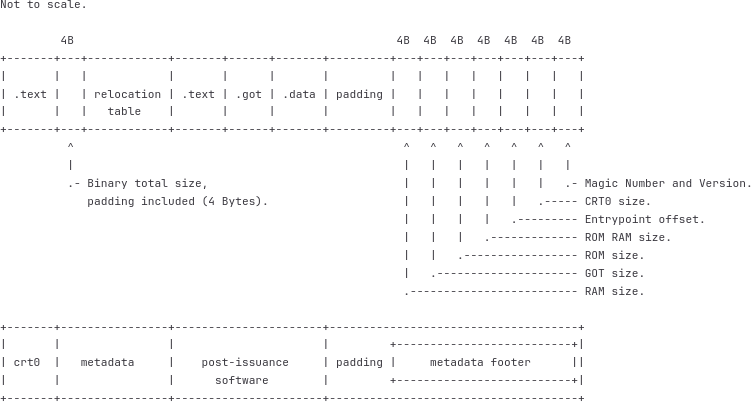
\includegraphics[width=\textwidth]{FAE_file_format.png}
    \caption{Detailed sections and software components diagrams}
\end{figure}

\subsection{Runtime processing}

Processing a FAE file has been designed to be as simple as possible.
From a high perspective point of view, it involves 4 entities performing sequential branches in the flow of execution.

First, a \texttt{caller site} branches to the first bytes of a FAE file, passing a context data structure as a parameter according to the ABI.
This context describes memories layout and stores executable arguments in a broader sense.

As seen in the file format description, this first branch leads to the \texttt{CRT0} location in FAE files, and more precisely to the \textit{\_start} function, thanks to the related linkscript.
From here, relying onto both FAE file's metadata section and metadata footer, \texttt{CRT0} performs :
\begin{itemize}
    \item runtime checks,
    \item memory initialization,
    \item all necessary relocations,
    \item and context updates.
\end{itemize}
When these steps are completed, \texttt{CRT0} finally retrieves the \texttt{post-issuance software entrypoint}, and branches to this address with the context data structure as a parameter.

The \texttt{post-issuance software entrypoint} is the same for all FAE files.\\
This code is in charge to initialize the software environment from the context data structure, before properly calling the specific \texttt{main} function it has been linked against.

Lastly, after the main returns, the flow of execution is restored back to the \texttt{caller site} thanks to the appropriate provided \textit{exit} function set in the software environment.

\subsubsection{Caller site}
\texttt{Caller sites} role is to initiate the FAE files execution process, by setting the Program Counter/Instruction Pointer CPU register to the FAE file starting memory address in ROM.
At the same time, \texttt{caller sites} must provide a context data structure according to the related \texttt{A}pplication \texttt{B}inary \texttt{I}nterface.

\paragraph{Context}
This data structure stores memory information such as :
\begin{itemize}
    \item the start address of the FAE file binary data in ROM,
    \item both available RAM start and end addresses,
    \item both free ROM start and end addresses,
    \item a generic pointer to arguments.\\
        Caller and callee must agree on a common arguments type.
        In regular FAE files, this type is a structure containing :
        \begin{itemize}
            \item the FAE file start address within the caller filesystem,
            \item a boolean flag indicating the execution takes place in a memory guarded environment,
            \item a table of functions pointers defining an API shared between the caller site and the post-issuance software.
            This allows to provide caller functionalities to software, the first notable one being the \textit{exit} function used at the end of the software entrypoint to return to callers.
            \item the command line arguments count,
            \item the command line arguments, as a C strings array,
            \item the address of the caller GOT, used by the post-issuance software before calling a shared API entry.\\
                    Callers are responsible for setting this field before branching into FAE file.
            \item the address of the post-issuance software GOT, used after having called a shared API entry.\\
                    CRT0 is responsible for setting this field before branching to the software entrypoint.
        \end{itemize}
\end{itemize}

\textit{
For the record, FAE file format is also used in several PIP-MPU related projects, namely "RIOT over PIP" and "pip-mpu-armv7-launcher".
In those cases, a dedicated CRT0 is embedded and the arguments type is a structure collecting the Root Partition information, ie :
\begin{itemize}
    \item partition descriptor block id,
    \item stack limit and top addresses,
    \item VIDT start and end addresses,
    \item the start address of the partition binary in ROM.
\end{itemize}
}

\subsubsection{CRT0 walkthrough}
CRT0 code begins with retrieving a pointer to the FAE file metadata section, thanks to the \textit{\_\_metadataOff} symbol set by CRT0 linkscript right after \textit{start} and \textit{text} sections.

From this, CRT0 computes the end of the file thanks to the ROM binary start address stored in context, and the binary size hosted in metadata section.
Now, CRT0 is able to access to the metadata footer information.

The next step is to check the \textit{Magic Number and Version} against CRT0 expected ones.
On failure, CRT0 prints an error message via semihosting, and terminates in an endless loop.

Otherwise, \textit{entrypoint offset, rom, got, data and bss sections sizes} are extracted from the metadata footer.
At this point, the respective sections start and entrypoint addresses in ROM are calculated.
Please note that regarding to \textit{rom} section, the FAE file \textit{optional padding} is skipped when found.

Then, CRT0 relies onto RAM start address stored in the context and the aforementioned sections size, to define the relocated segments addresses in RAM.
The relocated got segment address is assigned to the context field \textit{"current got"}.\\
The relocated segments addresses are checked against RAM start and end as defined in the context, to assert there is enough available RAM at runtime.
On failure, an error message is outputted via semihosting, and code terminates.

On success, both context's RAM and ROM start addresses are updated.
The data section contents are copied from ROM to RAM, and the bss segment is initialized to zero.\\
Immediately after, CRT0 relocates the got section entries from ROM to RAM.
Please note that each relocated entry address is checked against the respective relocated segment boundaries.
Once again, a faulty address leads to an error message and processing termination.

The relocation process ends with the table found in the FAE file metadata section.
The only supported cases are :
\begin{itemize}
    \item data entry referencing a data value,
    \item data entry referencing a bss value,
    \item data entry referencing a ROM value.
\end{itemize}

At last, CRT0 calls post-issuance \textit{software entrypoint}, with the updated context passed as a parameter according to the ABI.

\subsubsection{Software entrypoint}
The software entrypoint is also known as the \texttt{start} function; \textit{Please mind the missing '\_' character}.

At this stage, the API shared between callers and executables is fetched from the context and set in the software environment.\\
This is a collection of C function pointers depicting a functionalities set, originated from callers space, aimed at being called
in post-issuance software, through wrappers wherein both context's current and former got addresses are used.

Once the API set in the environment, the actual \textit{main} function is called with the \textit{arguments} and \textit{arguments count} stored in context.

Finally, on \textit{main} return, the flow of execution is routed back to callers thanks to the shared API function entry \textit{exit}, optionaly
with a return value where applicable.


\end{document}
